\documentclass{article}
\usepackage{../fasy-hw}
\usepackage{ wasysym }
\usepackage{fancyvrb}

%% UPDATE these variables:
\renewcommand{\hwnum}{3}
\title{Advanced Algorithms, Homework \hwnum}
\author{Nathan Stouffer \and Kevin Browder}
\collab{n/a}
\date{due: 17 September 2020}

\begin{document}

\maketitle

\nextprob
\collab{Nathan Stouffer and Kevin Browder}

Work in a group of size $\geq 2$.  Explain your strategy for working in a group.

\paragraph{Answer}

% ============================================

Our strategy for working in a group: we meet early in the week and work over the problems on scratch paper very informally. Doing this early will give us some extra time if there are any very difficult/time consuming problems Once we are satisfied with our work we do the LaTeX separately on our own time and use Git to collaborate on it. We then meet again before the assignment is due and go over the finished document and make sure everything looks good and we didn't make any mistakes when doing the LaTeX.

% ============================================

\nextprob
\collab{Nathan Stouffer and Kevin Browder}

Your group should make at least five contributions to the Piazza board.  A
contribution can be either asking a relevant question, responding to another
student's question, responding to an instructor's question, or choosing a
question from Chapter 1 and attempting to solve it, then  describing where you
get stuck in answering it.

\paragraph{Answer}

% ============================================

Our groups contributions are:
\begin{enumerate}
    \item (3-4, Kevin Browder, and 7:13pm-9/14/2020).

    As we learned in CS Theory a subset sum problem, which doesn't have a weight array is NP-Complete. Does the weight component of this problem change that? We think that it does because computing a maximum seems like it requires computing all the options to know for sure that we have the maximum.
    \item (3-3, Nathan Stouffer, 9:34am-9/15/2020).

    Hello everyone,

    Some languages (like java, c, c++ ...) allow any boolean condition to be a test for whether the loop should continue running and also allow any incrementing function. However, the examples that I have seen in this class seem to have a for loop running over a set of integers. Does the real-ram model allow for for loops that have a condition like end > beg with some specified incrementing function?

    The reason I ask is because of hw problem 3-3. The question asks that we write an algorithm for binary search using a for loop instead of recursion. If we must run over a set of integers, we can compute an upper bound on how many iterations the for loop will run so it is possible to create a correct for loop. I also think proving termination would be easier when running over a set of integers. However, the first option would be able to exit the for-loop before reaching the upper bound of iterations. This would not improve worst case run time but it would affect the average case run time. Let me know what we are allowed to do with this model of computation.

    Another idea would be to break out the loop if a certain condition is true. Is this allowable with our model of computation?

    \item (Problem 3-4 (response to a question from Dr. Fasy), Nathan Stouffer, and 10:30-9/15/2020). TODO:
        copy the post here.

        I can see how an answer to W would provide an answer to S. If we set all the weights equal to 0, then W is pretty much just S because we only need to find one subset of X that sums to T and it is guaranteed to be the maximum weight. So I agree that W is at least as difficult as S.

        If I remember things correctly, to show that W is NP-C, we would then want to show that W is a member of NP. In the theory course, that meant giving some Nondeterministic Polynomial Decider for W. But that was when everything was a decision problem. I'm not sure how things change when we switch to the real-ram model/are trying to optimize something. If giving some nondeterministic polynomial machine that solve W suffices to show that W is a member of NP, then the following machines might do that. \\

        SUBSETWEIGHT: \\
        Suppose we are given X, W, T.\\
        1. nondeterministically choose X' a subset of X\\
        2. if (sum the values of X' equals T)\\
        3.     weight = weight of X'\\
        4.     return weight\\
        5. else\\
        6.     return -inf\\

        MAXSUBSETWEIGHT:\\
        Suppose we are given X, W, T\\
        1. weights = SUBSETWEIGHT(X, W, T)\\
        2. return max { weights }\\

        I'm not really sure if all of this is allowable/fits under the span of the real-ram model. But it's what came to mind.

    \item (Problem 3-6 (Response to another students question), Kevin Browder, and 12:12-9/17/2020). I walked through the recursive calls like we did on Tuesday in class and used the Verbatim package in Latex for the indentation and to make it look at little nicer.
    \item (TODO: state the problem number, name of poster, and date/time). TODO:
        copy the post here.
\end{enumerate}

% ============================================

\nextprob
\collab{Nathan Stouffer and Kevin Browder}

Give the algorithm for binary search, using a for loop and no recursion.

\begin{enumerate}
    \item Describe the problem in your own words, including describing what the input and output is.
    \item Describe, in paragraph form, the algorithm you propose.
    \item Provide this algorithm in the algorithm environment.
    \item Use a decrementing function to prove that the loop terminates.
    \item What is the loop invariant? Provide the proof.
\end{enumerate}

\paragraph{Answer}

% ============================================

\begin{enumerate}
    \item The problem that binary search solves is returning the location of a target value in an array.
    The input to the problem must be a sorted array of comparable items paired with a target value of the same type.
    The output will either by the index of the target value or -1 to flag that the target is not in the array.
    \item
    \item Here is the algorithm.
    \begin{algorithm}
    	\textsc{BinarySearch}(A[1..n], targ) \\
    	1.  \hspace{0em}   beg $\leftarrow$ 1 \\
    	2.  \hspace{0em}   end $\leftarrow n$ \\
        3.  \hspace{0em}   indx $\leftarrow$ -1 // assume value is not in array \\
    	4.  \hspace{0em}   for $1.. \lceil log_2(len(A)) \rceil$ \\
    	5.  \hspace{2em}       mid $\leftarrow \lfloor (\text{beg}+\text{end})/2 \rfloor$ \\
    	6.  \hspace{2em}	   if (A[mid] = targ) \\
    	7.  \hspace{4em}	       indx $\leftarrow$ mid \\
    	8.  \hspace{2em}	   if (A[mid] $>$ targ) \\
    	9.  \hspace{4em}		   end $\leftarrow$ mid - 1 \\
    	10. \hspace{1.5em}	   if (A[mid] $<$ targ) \\
        11. \hspace{3.5em}        beg $\leftarrow$ mid + 1 \\
        12. return indx
    \end{algorithm}
    \item  This algorithm at its most basic level only iterates through the array. Every time it loops the array is cut in half. A array cannot be infinite because each index in an array is assigned to a memory location.  There is no such thing as infinite memory so therefore the length of an array is finite.  Since we are cutting the array in half every iteration the loop will run at most $log_2(len(A))$ times and since the length of A is finite the algorithm must terminate.
    \item Our loop invariant is that $arr[beg] < targ < arr[end]$.

\end{enumerate}

% ============================================

\nextprob
\collab{Nathan Stouffer and Kevin Browder}

Chapter 2, Problem 1b (Generalized \textsc{SubsetSum}).
\begin{enumerate}
    \item Describe the problem in your own words, including
        describing what the input and output is.
    \item Describe, in paragraph form, the algorithm you propose.
    \item Provide this algorithm in the algorithm environment.
    \item What is the runtime of your algorithm?
    \item Prove partial correctness (that if your algorithm terminates, it is
        correct).
\end{enumerate}


\paragraph{Answer}

% ============================================

\begin{enumerate}
    \item For the Generalized \textsc{SubsetSum} problem, our input has two parts.
    First, we have two equally sized arrays $X$ and $W$ containing positive integers paired with another positive integer $T$.
    Each value of $X$ has a corresponding weight in $W$ that can be found at the same index (ie weight for $X[i]$ can be found at $W[i]$).
    The second part of the input is an array called $I$ (which has length $len(X)$ and begins consisting entirely of 0s) paired with an index $i$ (which starts at 1).
    If it exists, our task is to find the subset of $X$ that sums to $T$ with the heaviest weight.
    If no subset of $X$ sums to $T$, we will return $-\infty$.
    Our output will either be $-\infty$ or a positve integer (the weight of the heaviest subset that sums to $T$).
    \item algorithm description \\
    The array $I$ contains activations for whether to include the $i^{th}$ element of $X$ in the subset (0 means don't include, 1 means include).
    The index i denotes the first index of $I$ that has not been yet been called.
    \item Here is the algorithm.
    \begin{algorithm}
        \textsc{SubsetSum}$(X, W, T, I, i)$ \\
        1.  \hspace{0em} if ($i > len(I)$) \\
        2.  \hspace{2em}     return $-\infty$ \\
        3.  \hspace{0em} if (\textsc{Sum}$(X, I) > T$) \\
        4.  \hspace{2em}     return $-\infty$ \\
        5.  \hspace{0em} if (\textsc{Sum}$(X, I) = T$) \\
        6.  \hspace{2em}     return \textsc{Weight}($W, I$) \\
        7.  \hspace{0em} skip $\leftarrow$ \textsc{SubsetSum}($X, W, T, I, i+1$) \\
        8.  \hspace{0em} $I[i] \leftarrow 1$ \\
        9.  \hspace{0em} take $\leftarrow$ \textsc{SubsetSum}($X, W, T, I, i+1$) \\
        10. return max(skip, take) \\

        \textsc{Sum}(X, I) \\
        1.  \hspace{0em} sum $\leftarrow$ 0 \\
        2.  \hspace{0em} for i in 1..len(X) \\
        3.  \hspace{2em}     sum $\leftarrow$ sum + $X[i]*I[i]$ \\
        4.  \hspace{0em} return sum \\

        \textsc{Weight}(W, I) \\
        1.  \hspace{0em} weight $\leftarrow$ 0 \\
        2.  \hspace{0em} for i in 1..len(W) \\
        3.  \hspace{2em}     weight $\leftarrow$ weight + $W[i]*I[i]$ \\
        4.  \hspace{0em} return weight
    \end{algorithm}
    \newpage
    \item Towards giving the runtime of our algorithm, we start by giving the run times of \textsc{Sum} and \textsc{Weight}.
    Let $n$ be the length of $X$ (which matches the lengths of $W$ and $I$).
    Both \textsc{Sum} and \textsc{Weight} run in $\Theta(n)$ (since they have constant time operations that run $n$ times).
    Now we give the worst case recurrence relation for \textsc{SubsetSum}: $T(n) = \Theta(n) + \Theta(n) + T(n-1) + O(1) + T(n-1) = 2*T(n-1) + \Theta(n)$.
    We can then say that $T(n) = O(2^n)$.
    \item First we set up the recursive invariant: The initialization step is checking to see if $i$ is greater than the length of $I$ or if the sum of $X$ and $I$. If either of these are true we return $-\infty$. The maintenance step is checking if the sum of $X$ and $I$. This means that every time we make the recursive call we move up the $X$ array.  Using strong induction, we have the base case were the sum of $X$ and $I$ is equal to $T$.  Our inductive hypothesis: We assume that the recursive invariant holds true for all previous recursive steps.  As our inductive step, since we assume the inductive hypothesis, we then check both variations of $I$ (0, 1). So, by induction, we have proven that the algorithm is correct.
\end{enumerate}

% ============================================



\nextprob
\collab{Nathan Stouffer and Kevin Browder}

Describe two different data structures that you can use to store a graph.
Please give a complete description (i.e., a response of ``an array'' will not
suffice).

\paragraph{Answer}

% ============================================

\begin{enumerate}
	\item Array: Use a two dimensional array of nodes to create an adjacency matrix. Edges are represented by non-zero values in the array. The size of the matrix is a square where the width and height are the number of nodes. \\
	Example: 0--1--2\\
	Adjacency Matrix:\\
	$\{\{0, 1, 0\}\\$
	$\{1, 0, 1\}\\$
	$\{0, 1, 0\}\}\\$

	\item Adjacency List: Use an array of lists where each index of the array is a vertex. At each index in the array (array[i]) there is a list of nodes that are adjacent to the ith node. \\
	Example: 0--1--2\\
	$\{[1],$\\
	$[[0],[2]],$\\
	$[1]\}$\\

	\item Relational Database: Have a node table and an edge table. The node table has a node ID and the edges table consists of two rows, A and B. Which contain the start and end node ID's of an edge respectively. This works best for directed graphs.
	Example: 0--1--2\\

	\begin{table}[H]
		\begin{tabular}{|l|l|l|}
			\hline
			ID & Name   & Feature \\ \hline
			0  & Node 0 & A       \\ \hline
			1  & Node 1 & A       \\ \hline
			2  & Node 2 & B       \\ \hline
		\end{tabular}
	\end{table}
	\begin{table}[H]
		\begin{tabular}{|l|l|}
			\hline
			A & B \\ \hline
			0 & 1 \\ \hline
			1 & 0 \\ \hline
			1 & 2 \\ \hline
			2 & 1 \\ \hline
		\end{tabular}
	\end{table}
\end{enumerate}

% ============================================


\nextprob
\collab{Nathan Stouffer and Kevin Browder}

Walk through the exponential time Longest Increasing Subsequence (LIS) algorithm
on page 108 for the input: $\left[ 1, 7, 6, 11, 3, 11 \right]$.



Walk through the algorithm using the Dynamic Programming algorithm present in
Section 3.6.1

\paragraph{Answer}

% ============================================

\begin{enumerate}
	\item 
	\begin{figure}[h]
		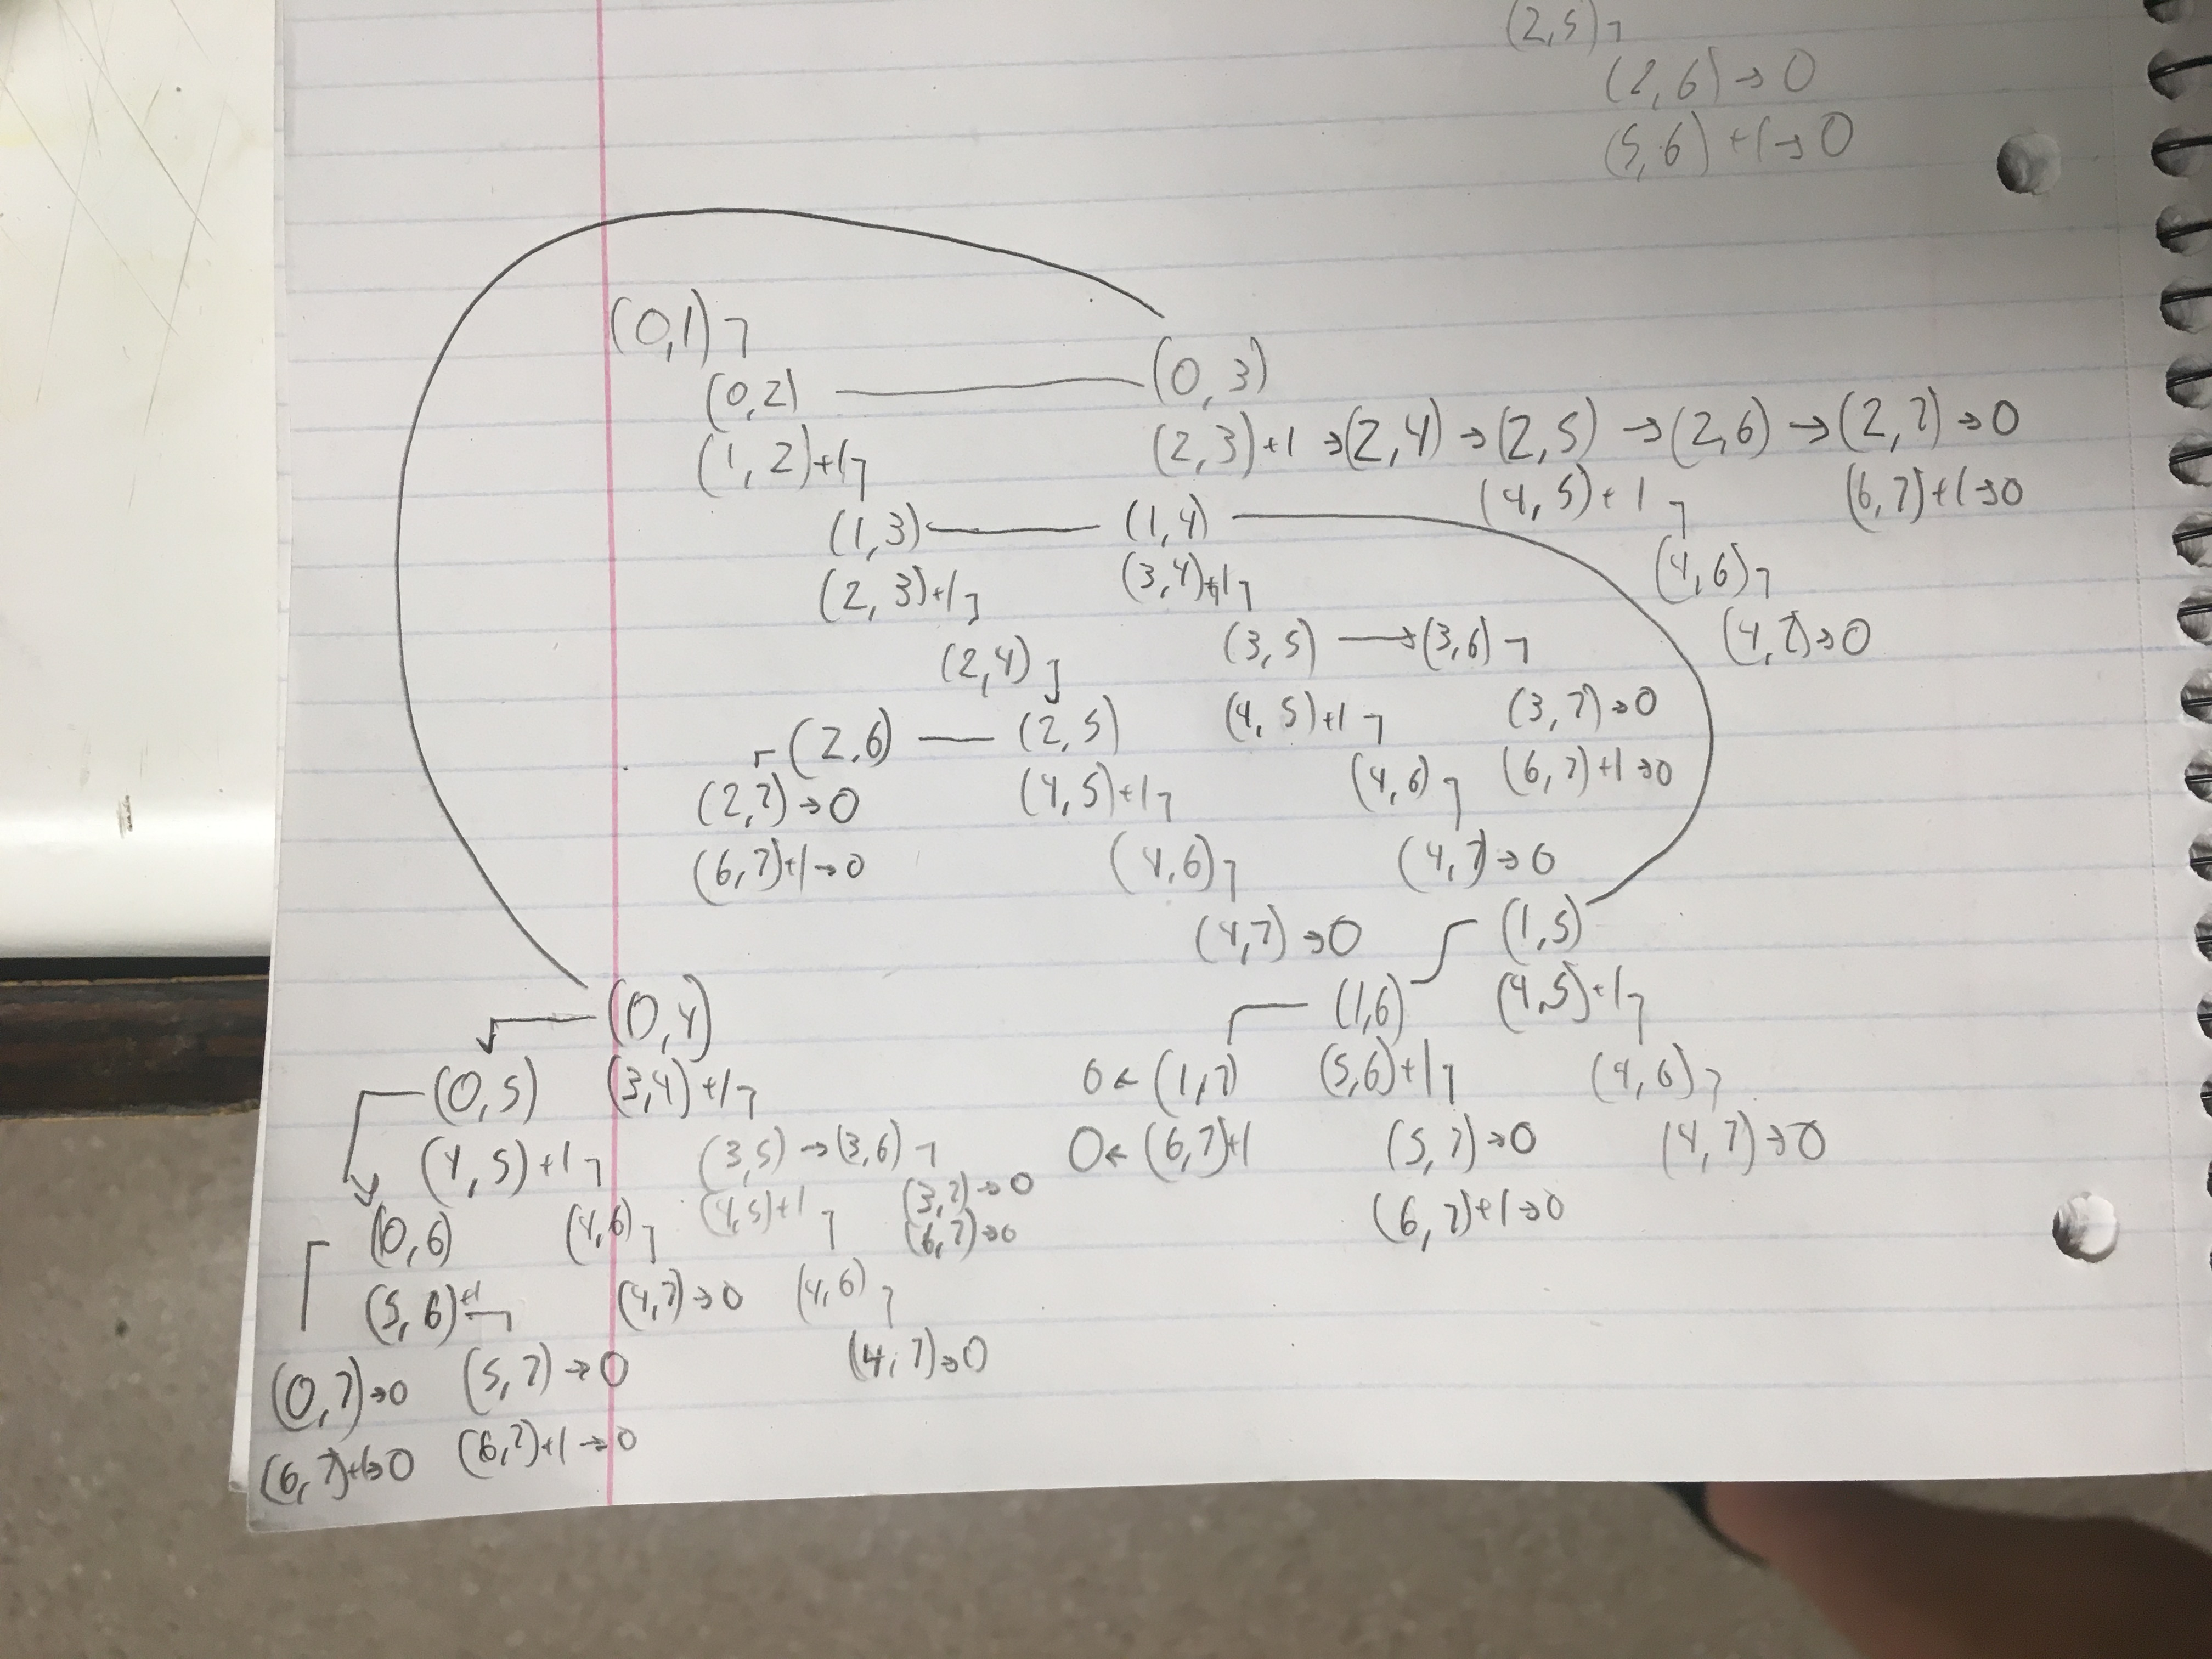
\includegraphics[width=\linewidth]{image0.jpeg}
		\caption{Problem 6 Part 1}
		\label{fig:q1class}
	\end{figure}
\end{enumerate}

% ============================================

\nextprob
\collab{Nathan Stouffer and Kevin Browder}

What is the closed form of the following recurrence relations?  Use the master
theorem to justify your answers:
\begin{enumerate}
    \item $T(n) = 16 T(n/4) + \Theta(n)$
    \item $T(n) = 2 T(n/2) + n \log{n}$
    \item $T(n) = 6 T(n/3) + n^2 \log{n}$
    \item $T(n) = 4 T(n/2) + n^2$
    \item $T(n) = 9 T(n/3) + n$
\end{enumerate}
Note: we assume that $T(1)=\Theta(1)$ whenever it is not explicitly given.

\paragraph{Answer}

% ============================================

\begin{enumerate}
    \item Our recurrence relation is $T(n) = 16T(n/4) + \Theta (n)$.
    In the context of the master theorem, $f(n) = \Theta (n)$ and $n^{\log_b a} = n^{\log_4 16} = n^2$.
    We claim this fits case 1 of the master theorem.
    To show this, we must show that (for some $\epsilon > 0$) $f(n) = O(n^{\log_b a - \epsilon}) \iff \Theta (n) = O(n^{2 - \epsilon})$. \parspace
    Choose $\epsilon = 1$ and then we have $\Theta (n) = O(n)$ which is true if and only if $O(n) = O(n)$ and $n = O(n)$ (this is by definition of big-theta).
    The first equality is trivially true and take $n_0 = 1$ and $c = 1$ to show that the second equality holds. \parspace
    Thus, $T(n)$ satisfies case 1 of the master theorem and $T(n) = \Theta (n^2)$.
    \item Our recurrence relation is $T(n) = 2T(n/2) + n \log n$.
    In the context of the master theorem, $f(n) = n \log n$ and $n^{\log_b a} = n^{\log_2 2} = n^1 = n$.
    We claim this fits case 3 of the master theorem.
    To show this, we must show that $f(n) = \Omega (n^{\log_b a + \epsilon})$ for $\epsilon > 0$ and $a f(n/b) \leq c_1 f(n)$ for some $c_1 > 1$. \parspace
    We first show that $f(n) = \Omega (n^{\log_b a + \epsilon}) \iff n \log n = \Omega (n^{1 + \epsilon}) \iff n^{1 + \epsilon} = O(n \log n)$.
    Choose $\epsilon = ?$
    So we must show $n^ = O(n \log n)$.
    Choose
    \item Our recurrence relation is $T(n) = 6T(n/3) + n^2 \log n$.
    In the context of the master theorem, $f(n) = n^2 \log n$ and $n^{\log_b a} = n^{\log_3 6}$ (note that $\log_3 6 \in (1,2)$).
    We claim this fits case 3 of the master theorem.
    To show this, we must show that $f(n) = \Omega (n^{\log_b a + \epsilon})$ for $\epsilon > 0$ and $a f(n/b) \leq c_1 f(n)$ for some $c_1 > 1$. \parspace
    We first show that $f(n) = \Omega (n^{\log_b a + \epsilon}) \iff n^2 \log n = \Omega (n^{\log_3 6 + \epsilon}) \iff n^{\log_3 6 + \epsilon} = O(n^2 \log n)$.
    Choose $\epsilon$ such that $\log_3 6 + \epsilon = 2$.
    So we must show $n^2 = O(n^2 \log n)$.
    Choose $n_0 = 2$ and $c_0 = 1$, then we verify that $n^2 \leq 1 n^2 \log n$ for all $n \geq 2$.
    Consider, $ n^2 \leq 1 n^2 \log n \iff 1 \leq \log n $ which is certainly true for for all $n \geq 2$. \parspace
    We must now show that $6 f(n/3) \leq c_1 f(n)$ for some $c_1$ and sufficiently large $n$.
    Choose $c_1 = 2$.
    $$ 6 f(n/3) \leq c_1 f(n) \iff 6 (n/3)^2 \log(n/3) \leq 2 n^2 \log(n) \iff (2/3) \log (n/3) \leq 2 \log (n) $$
    Using properties of logarithms, we can equivalently say that $\log ((n/3)^{2/3}) \leq \log (n^2)$ which is true exactly when $(n/3)^{2/3} \leq n^2 \iff n/3 \leq n^3 \iff 1/3 \leq n^2$ which is true for $n \geq 1/\sqrt{3}$. \parspace
    Therefore, $T(n)$ satisfies case 3 of the master theorem and $T(n) = \Theta (n^2 \log n)$.
    \item Our recurrence relation is $T(n) = 4T(n/2) + n^2$.
    In the context of the master theorem, $f(n) = n^2$ and $n^{\log_b a} = n^{\log_2 4} = n^2$.
    We claim this satisfies case 2 of the master theorem.
    To show this, we must show that $f(n) = n^2 = \Theta (n^{\log_b a}) = \Theta (n^2)$. \parspace
    To show that $n^2 = \Theta (n^2)$, we must show that $n^2 = O(n^2)$ (showing the other case is symmetric so there is only the condition).
    Choose $n_0 = 1$ and $c = 1$, then $n^2 \leq n^2$ for all $n > 1$ and we conclude that $n^2 = O(n^2)$. \parspace
    So $T(n)$ satisfies case 2 of the master theorem and $T(n) = \Theta (n^2 \log n)$.
    \item Our recurrence relation is $T(n) = 9T(n/3) + n$.
    In the context of the master theorem, $f(n) = n$ and $n^{\log_b a} = n^{\log_3 9} = n^2$.
    We claim this satisfies case 1 of the master theorem.
    To show this, we must show that $f(n) = n = O(n^{\log_b a - \epsilon}) = O(n^{2 - \epsilon})$ for some $\epsilon > 0$. \parspace
    Let $\epsilon = 1$, then we must show that $n = O(n)$.
    Choose $c = 1$ and $n_0 = 1$.
    Then $n \leq n \iff 1 \leq 1$ which is certainly true for all $n \geq 1 = n_0$.
    So $T(n)$ satisfies case 1 of the master theorem and $T(n) = \Theta (n^2)$.
\end{enumerate}

% ============================================

\nextprob
\collab{Nathan Stouffer and Kevin Browder}

\emph{The skyline problem:} You are in Camden, NJ waiting for the ferry across the river to
get into Philadelphia, and are looking at the skyline.  You take a photo, and notice that each building
has the silhouette of a rectangle.  Suppose you  represent each building $b$ as a
triple $(x_b^{(1)},x_b^{(2)},y_b)$, where the building can be seen from $x_b^{(1)}$ to $x_b^{(2)}$
horizontally and has a height of $y_b$.  Let $\mathtt{rect(b)}$ be the set of
points inside this rectangle (including the boundary).  Let $\mathtt{buildings}$
be a set of $n$ such triples representing buildings. Design an algorithm that takes $\mathtt{buildings}$ as input, and
returns the skyline, where the skyline is a sequence of~$(x,y)$ coordinates
defining $\cup_{b \in \mathtt{buildings}} \mathtt{rect}(b)$.  The output should
start with $(\min_b{x_b^{(1)}},0)$ and end with $(\max_b{x_b^{(2)}},0)$.

\begin{enumerate}
    \item Describe the problem in your own words, including describing what the input and output is.
    \item Describe, in paragraph form, the algorithm you propose.
    \item Provide this algorithm in the algorithm environment.
    \item What is the runtime of your algorithm? If you do not know, either give the tightest bounds you know, or provide a decrementing function to show that it does terminate.
    \item Prove partial correctness (that if your algorithm terminates, it is correct).
\end{enumerate}

\paragraph{Answer}

% ============================================

\begin{enumerate}
    \item
    \item
    \item Here is our algorithm.
    \begin{algorithm}
        \textsc{Skyline}(buildings) \\
        1. \hspace{0em} sorted $\leftarrow$ \textsc{SortByX1}(buildings) \hspace{2em} // buildings sorted by $x_b^{(1)}$ \\
        2. \hspace{0em} lastx $\leftarrow$ \textsc{SortByX2}(buildings)[len(buildings)] \hspace{2em} // get the largest $x_b^{(2)}$\\
        3. \hspace{0em} x $\leftarrow$ buildings[1][1] \\
        4. \hspace{0em} y $\leftarrow$ \textsc{Height}(sorted, 0) \\
        5. \hspace{0em} skyline $\leftarrow$ (x, 0) $\cup$ (x, y) \hspace{2em} // list to store the skyline (we use union to represent appending) \\
        6. \hspace{0em} while (x $<$ lastx) \\
        7. \hspace{2em} newx $\leftarrow$ \textsc{NextX}(sorted, lastx, x, y) \hspace{2em} // get the x at the next intersection in the skyline \\
        8. \hspace{2em} skyline $\leftarrow$ skyline $\cup$ (newx, y) \hspace{2em} // draw a horizontal line \\
        9. \hspace{2em} newy $\leftarrow$ \textsc{Height}(sorted, newx) \hspace{2em} // get the y value for the skyline at newx \\
        10. \hspace{1.5em} skyline $\leftarrow$ skyline $\cup$ (newx, newy) \hspace{2em} // draw a vertical line \\
        11. \hspace{1.5em} x $\leftarrow$ newx \\
        12. \hspace{1.5em} y $\leftarrow$ newy \\
        13. skyline $\leftarrow \cup$ (lastx, 0) // since the loop has terminated, go straight down \\
        14. return skyline \\\\

        \textsc{Height}(sorted, x) \\
        1. \hspace{0em} height $\leftarrow$ 0 \\
        2. \hspace{0em} for i in $1..len(sorted)$ \\
        3. \hspace{2em}     if (sorted[i][1] $\leq$ x $<$ sorted[i][2]) \\
        4. \hspace{4em}         if (sorted[i][3] $>$ height) \\
        5. \hspace{6em}             height $\leftarrow$ sorted[i][3] \\\\

        \textsc{NextX}(sorted, lastx, x, y) \\
        1. \hspace{0em} next $\leftarrow$ lastx \\
        2. \hspace{0em} for i in $1..len(sorted)$ \\
        3. \hspace{2em}     candidate $\leftarrow$ sorted[i][1]\ \\
        4. \hspace{2em}     if (x $\leq$ candidate) \hspace{2em} // check if building starts after x \\
        5. \hspace{4em}         if (candidate $<$ next) \hspace{2em} // check if buiding is closer than current next \\
        6. \hspace{6em}              if (\textsc{Height}(sorted, candidate) $>$ \textsc{Height}(sorted, next)) \hspace{2em} // check if candidate is taller \\
        7. \hspace{8em}                  next $\leftarrow$ candidate \\
        8. \hspace{0em} return candidate
    \end{algorithm}
\end{enumerate}
% ============================================



\end{document}
